\section{Control via I/O feedback linearization}
From the control perspective, Ingenuity is an underactuated robot, since the number of control inputs is less than the number of degrees of freedom. Specifically, it has six degrees of freedom (three for the position and three for the orientation) and only four control inputs (the rotation speed of the two rotors $\omega_u$ and $\omega_l$, and the thrust vector angles $\alpha$ and $\beta$). 

In order for the robot to be controlled, it is necessary to exploit its natural dynamics by employing the four inputs  to impart a certain behavior to the total system (both positional and rotational state variables) such that, at the end of the day, the three-dimensional position and the yaw angle follow the desired course in time. To grasp the concept, the reader can imagine a quadrotor or helicopter with a tail rotor, which need to tilt in the desired direction in order to move.

If we choose as controlled outputs of the system the three position components and the yaw angle, it is possible to employ the input-to-output feedback linearization technique to design a controller that renders unobservable the nonlinear dynamics of the helicopter. As a result, the system seen between input and output will have linear dynamics and thus could be easily controlled via linear control techniques.

Consider the following nonlinear state-space representation of the robot dynamics:
\begin{align}
    \frac{d}{dt} \begin{bmatrix}
        P \\ V^b \\ W \\ \Omega^b
    \end{bmatrix} = \begin{bmatrix}
        R \, V^b \\ \frac{1}{m} R^T F_g^i -\Omega^b \times V^b + \frac{1}{m} u \\ R \, \Omega^b \\ -I^{-1} \Omega^b \times (I \Omega^b)+I^{-1}\tau_{tot}^b 
    \end{bmatrix}
    \label{eq:fbl_model}
\end{align}
where the input $u$ is the total thrust force generated by the rotors: 
\begin{align}
    u = F_u^b + F_l^b.    
    \label{eq:u} 
\end{align}
Calculations are facilitated if we make a change of coordinates to the inertial frame. 
$$ \frac{d}{dt} \begin{bmatrix}
    P \\ \dot{P}
\end{bmatrix} = \begin{bmatrix}
    \dot{P} \\ \frac{1}{m} F_g^i + \Omega^b \times \dot{P} - (R \Omega^b) \times \dot{P} + \frac{1}{m} R u
\end{bmatrix}. $$

The idea is to choose $u$ to cancel the nonlinear part of the positional dynamics:
$$u = m R^T [(R \Omega^b) \times \dot{P} - \Omega^b \times \dot{P} - \frac{1}{m} F_g^i + v].$$
The transfer function relating the input $v$ to the output $P$ is then a double integrator:
$$\frac{d^2}{dt^2} P(t) = v(t) \iff \frac{P(s)}{v(s)} = \frac{1}{s^2}.$$
It can be controlled using a simple PD controller with a feedforward term:
$$v = k_{p,1} (P_d - P) + k_d \bigg(\frac{d}{dt}P_d - \dot{P}\bigg) + \frac{d^2}{dt^2}P_d.$$

Notice that the only input affecting the $\Omega_3^b$ dynamics is the reaction torque $\tau_r^b$. Controlling the third component of the angular velocity in the body frame is all we can do if we want to keep the inputs $u$ and $\tau_r^b$ decoupled, and it is sufficient if we assume that the roll and pitch angles are sufficiently small. Therefore, we proceed in an analogous way to the previous case, choosing:

$$ \tau_r^b = \begin{bmatrix}
    0 & 0 & 0 \\ 0 & 0 & 0 \\ 0 & 0 & 1
\end{bmatrix}[\Omega^b \times (I \Omega^b) + I w]$$
This results in the following transfer function for the $\Omega_3^b$ dynamics:
$$\frac{d}{dt} \Omega_3^b(t) = w_3(t) \iff \frac{\Omega_3^b(s)}{w_3(s)} = \frac{1}{s},$$
where $w_3$ is the third component of $w$. The linearized system can be controlled using a simple proportional controller with a feedforward term:
$$w = \begin{bmatrix}
    0 \\ 0 \\k_{p,2} (\Omega_{3,d}^b - \Omega_3^b) + \frac{d}{dt}\Omega_{3,d}^b
\end{bmatrix} .$$

Following this, a critical point is reached: once an feedback linearizing control is implemented, it is worth taking a look at how the part of the system that has been hidden behaves. We could call this part, in a non-formal way, the \textit{forced zero dynamics} of the system. It is obtained by substituting \ref{eq:torque_due_force} and \ref{eq:torque} in \ref{eq:fbl_model}:
\begin{align*}
    \frac{d}{dt}\begin{bmatrix}
        \Omega^b_1 \\
        \Omega^b_2
    \end{bmatrix}
    = 
    \begin{bmatrix}
        -\frac{F_{l,2}^b d_{cm,l} + F_{u,2}^b d_{cm,u}}{I_{1,1}} - \frac{I_{2,2}-I_{3,3}}{I_{1,1}} \Omega^b_2 \Omega^b_3 \\
        \frac{F_{l,1}^b d_{cm,l} + F_{u,1}^b d_{cm,u}}{I_{2,2}} + \frac{I_{1,1}-I_{3,3}}{I_{2,2}} \Omega^b_1 \Omega^b_3
    \end{bmatrix}.
\end{align*}
The latter is an autonomous dynamics that is affected by the signals $F_{l,1}^b$, $F_{l,2}^b$, $F_{u,1}^b$ and $F_{u,2}^b$, which in turn depend on the feedback linearizing control. In practical terms, in order to enforce the designed behavior, the controller may induce pseudo-chaotic angular accelerations in the not-directly-controllable part of the system, leading to undesired and "clumsy" behaviors. It is a consequence of the fact that the system is underactuated.

\subsection{Actuation} \label{sec:fbl_actuation}
The objective of this section is to recover the actual control inputs of Ingenuity, i.e. the rotation speed of the upper and lower blades $\omega_u$ and $\omega_l$ and the tilt angles of the swashplate $\alpha$ and $\beta$, given the values of the linearizing signals $u$ and $\tau_{r}^b$ entering the system in \ref{eq:fbl_model} with \ref{eq:torque}.

Since \ref{eq:u} holds, from the definition of the angles $\alpha$ and $\beta$ illustrated in \ref{fig:alpha_beta}, under the assumption that $u_3 \neq 0$ \footnote{Always satisfied during normal conditions, since there will always be a part of $u_3$ counteracting gravity.}, the following is straightforward:
\begin{gather*}
    \alpha = \arctan\left(\frac{u_1}{u_3}\right), \\
    \beta = \arctan\left(\frac{u_2}{u_3}\right),
\end{gather*}
where $u_1$, $u_2$ and $u_3$ are the components of the vector $u$.

Knowing $\alpha$ and $\beta$, it is possible to combine the third component of \ref{eq:force} and \ref{eq:u} to find the sum of the norms of the forces $F_u^b$ and $F_l^b$, given that $\cos{\gamma} \neq 0$\footnote{Consequence of $u_3 \neq 0$\footnotemark[1] using \ref{eq:u} and \ref{eq:force}.}:
\begin{align*}
    ||F_u^b|| + ||F_l^b|| = \frac{u_3}{\cos{\gamma}},
\end{align*}
while their difference is given by exploiting \ref{eq:reaction_torque}:
\begin{align*}
    ||F_u^b|| - ||F_l^b|| = 50 \, \tau^b_{r,3},
\end{align*}
where $\tau^b_{r,3}$ is the third component of the vector $\tau^b_r$.\\
Using \ref{eq:force_norm}, we obtain the following system of equations:
\begin{equation*}
    \left\{\begin{array}{@{}l@{}}
        (K_l - K_d) \, (\omega_u^2 + \omega_l^2)= \frac{u_3}{\cos{\gamma}} \\
        (K_l - K_d) \, (\omega_u^2 - \omega_l^2) = 50 \, \tau^b_{r,3} \\
    \end{array}\right. ,
\end{equation*}
whose solutions are:
\begin{gather*}
    \omega_u = \sqrt{\frac{\frac{u_3}{\cos{\gamma}} + 50 \, \tau^b_{r, 3}}{2 \, (K_l - K_d)}}, \\
    \omega_l = \sqrt{\frac{\frac{u3}{\cos{\gamma}} - 50 \, \tau^b_{r, 3}}{2 \, (K_l - K_d)}}
\end{gather*}
and only exist if $\tau^b_{r, 3}$ satisfies:
\begin{align*}
    |\tau^b_{r, 3}| \leq \frac{u_3}{50 \, \cos{\gamma}}.
\end{align*}
\subsection{Simulation results} \label{sec:fbl_sim}
The implemented control law was tested on a trajectory tracking task. To complete the task, the helicopter is required to perform, cyclically with period $T = \qty{100}{\second}$, an helical trajectory for $\qty{70}{\second}$ and then to come back to the origin in the remaining $\qty{30}{\second}$, while keeping the yaw angle to zero, i.e.
\begin{align}
    &P^d=\begin{cases*}
        \begin{bmatrix}
            r\cdot cos(\frac{t}{d}) \\ r\cdot sin(\frac{t}{d})\\ 1+\frac{t}{k}
        \end{bmatrix} \quad &if $t$ \% 50 $<$ 30 \\
        \begin{bmatrix}
            0 \\ 0 \\ 0
         \end{bmatrix} \quad &else
    \end{cases*} \label{eq:pos_ref}\\
    &W^d=0 \label{eq:yaw_ref}
\end{align}

\noindent with $r=\qty{5}{\meter}$ radius of the helix, $d=5$ a scaling factor regulating the speed of the $(x,y)$ plane and $k=10$ a scaling factor regulating the rate of climb. The symbol $\%$ stands for remainder after division. \\
Moreover, the initial position of the robot belongs to the helical trajectory, while the initial attitude is null.

For the sake of realism, the control inputs to the system cannot range over an infinite span, but it is appropriate to constrain them to vary over limited intervals. More specifically, we impose the following constraints:

\begin{gather}
    \omega_u \in [0, 2800] \, \textit{rpm} \label{eq:omega_u_constraint} \\
    \omega_l \in [-2800, 0] \, \textit{rpm} \label{eq:omega_l_constraint} \\
    \alpha \in [-10, 10]^\circ \label{eq:alpha_constraint} \\
    \beta \in [-10, 10]^\circ \label{eq:beta_constraint}
\end{gather}

Figure \ref{fig:FL_trajectory} shows the comparison between the reference and the actual trajectory traversed by the robot. The tracking performance is outstanding as long as the error is small, but failure occurs in the instant that the error is too large, because of the explosion of the states governing the forced zero dynamics. We deduce that the system is extremely unrobust, so the control action is not sufficiently reliable.
\begin{figure}[H]
    \centering
    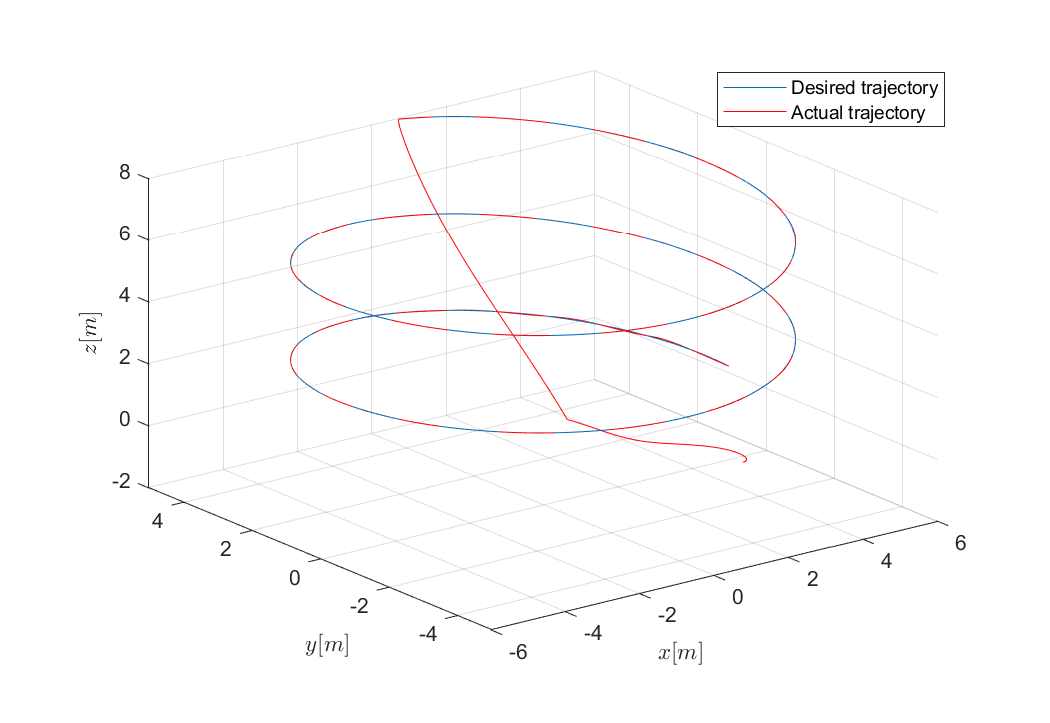
\includegraphics[scale=0.5]{figures/FL_trajectory}
    \caption{Trajectory tracking.}
    \label{fig:FL_trajectory}
\end{figure}
This phenomenon is also visible in Figure \ref{fig:FL_attitude}. Despite the pitch having, up to a certain point, an acceptable evolution, the roll exhibits noticeable fluctuations that induce Ingenuity to assume an unrealistic behavior. As an additional consequence, the small angles assumption of the previous signals is violated, leading to a significant error in the yaw angle, whose reference is not followed. Moreover, as in the previous graph, the abrupt change in the reference causes the bursting of the examined states.
\begin{figure}[H]
    \centering
    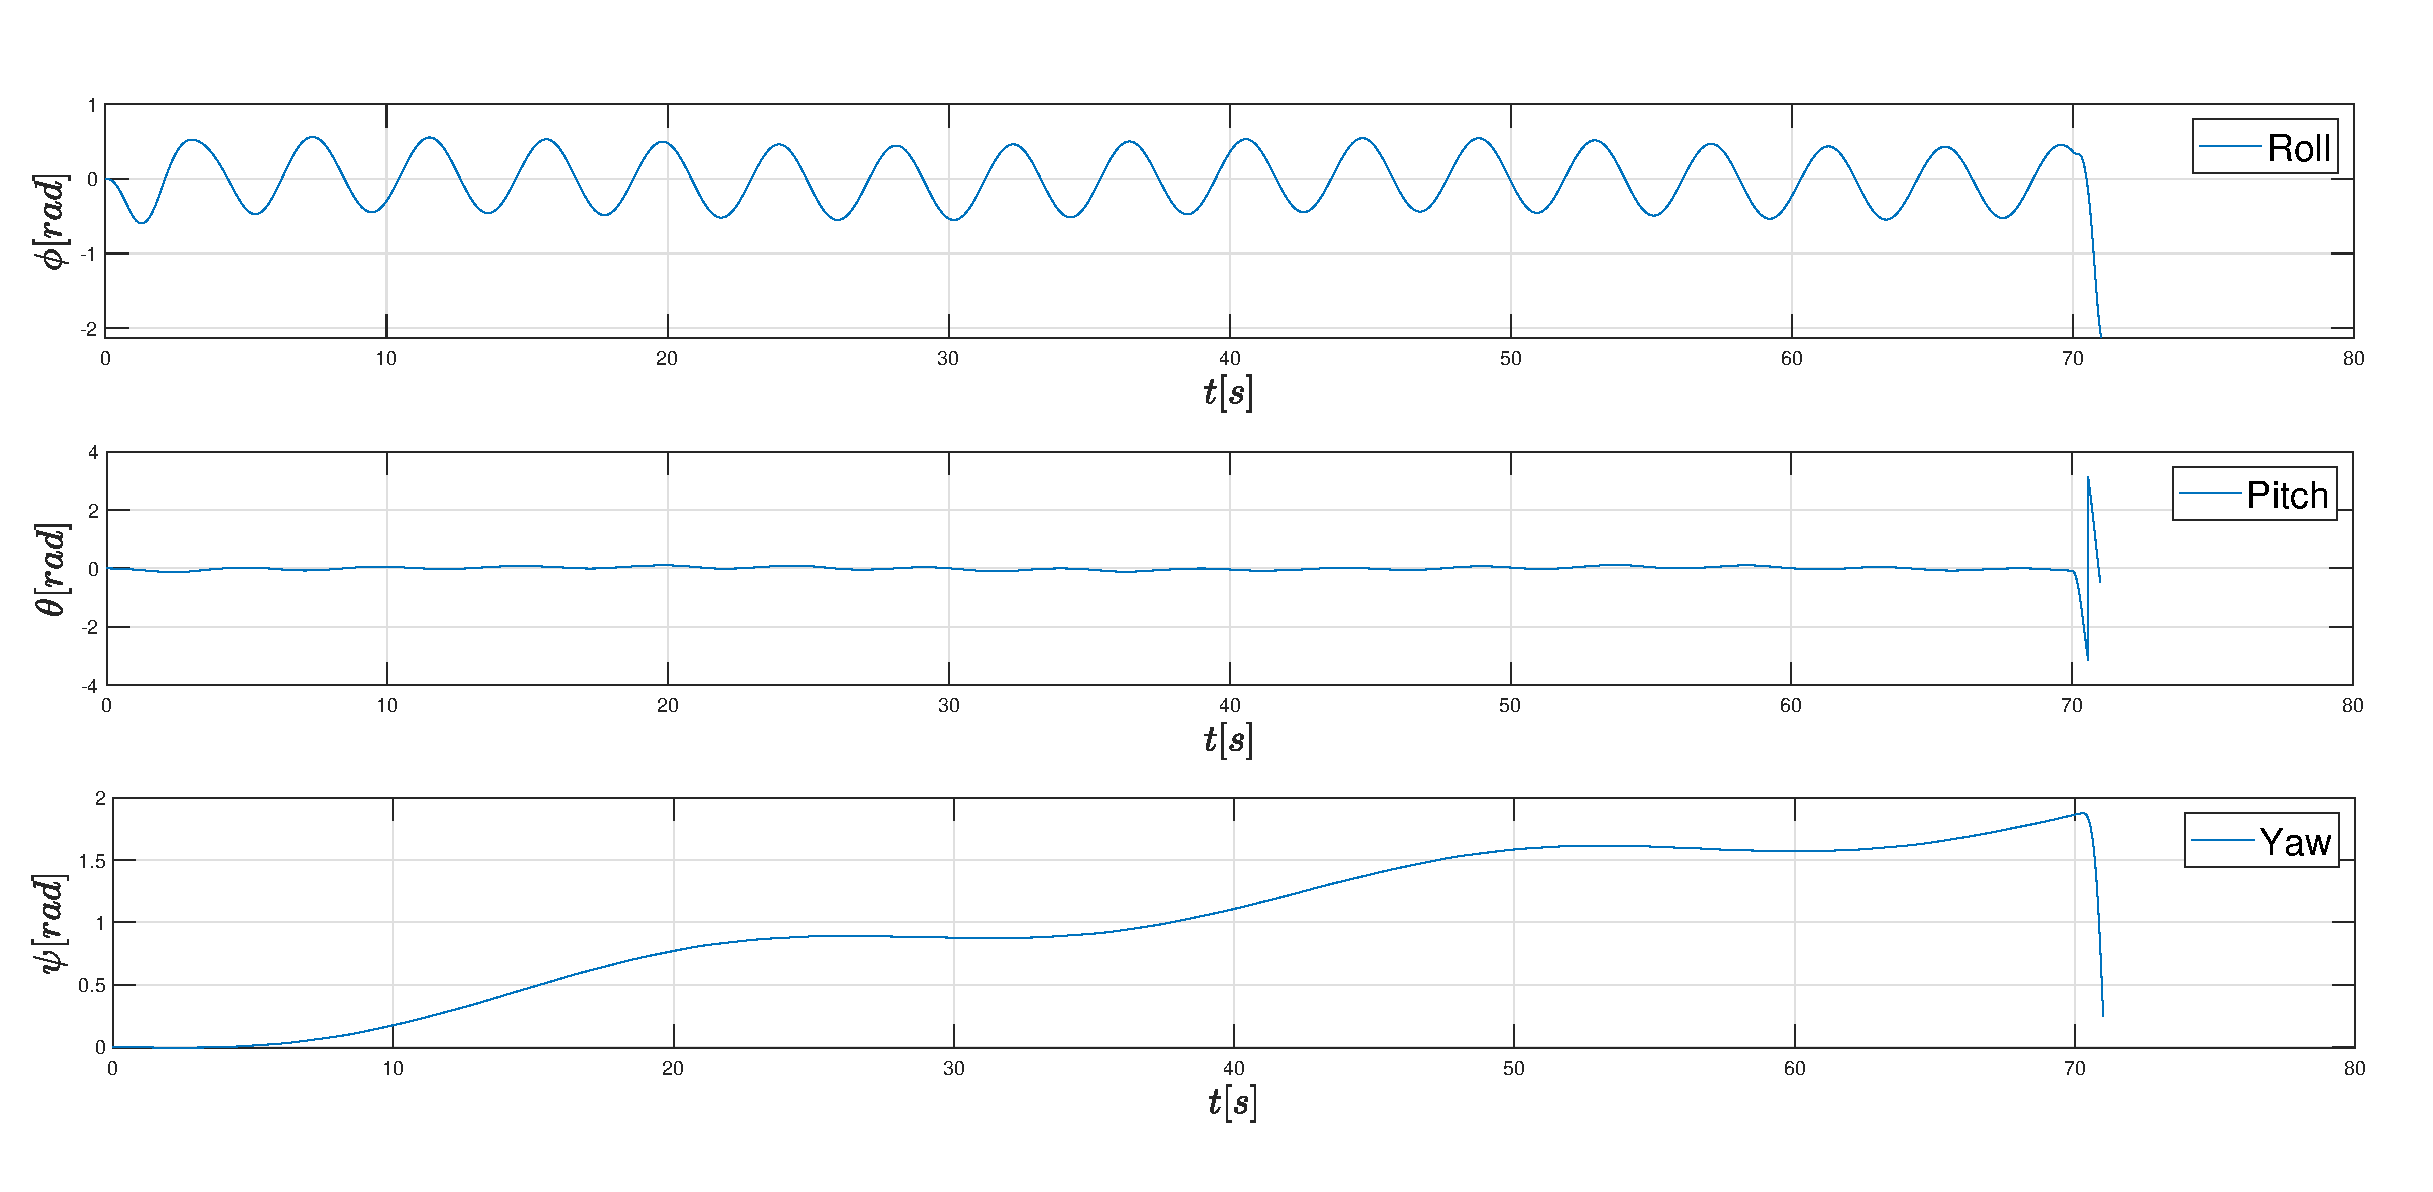
\includegraphics[scale=0.2]{figures/FL_attitude}
    \caption{Evolution of the roll, pitch and yaw angles respectively.}
    \label{fig:FL_attitude}
\end{figure}
The previous results can only be obtained if the inputs are not constrained. In fact, Figures \ref{fig:FL_angles} and \ref{fig:FL_omega} show that the value of the angle $\beta$ breaks the constraint \ref{eq:beta_constraint}. If saturations were imposed on the input signals, the system would fail to track the trajectory and diverge even in the initial phase.
\begin{figure}[H]
    \centering
    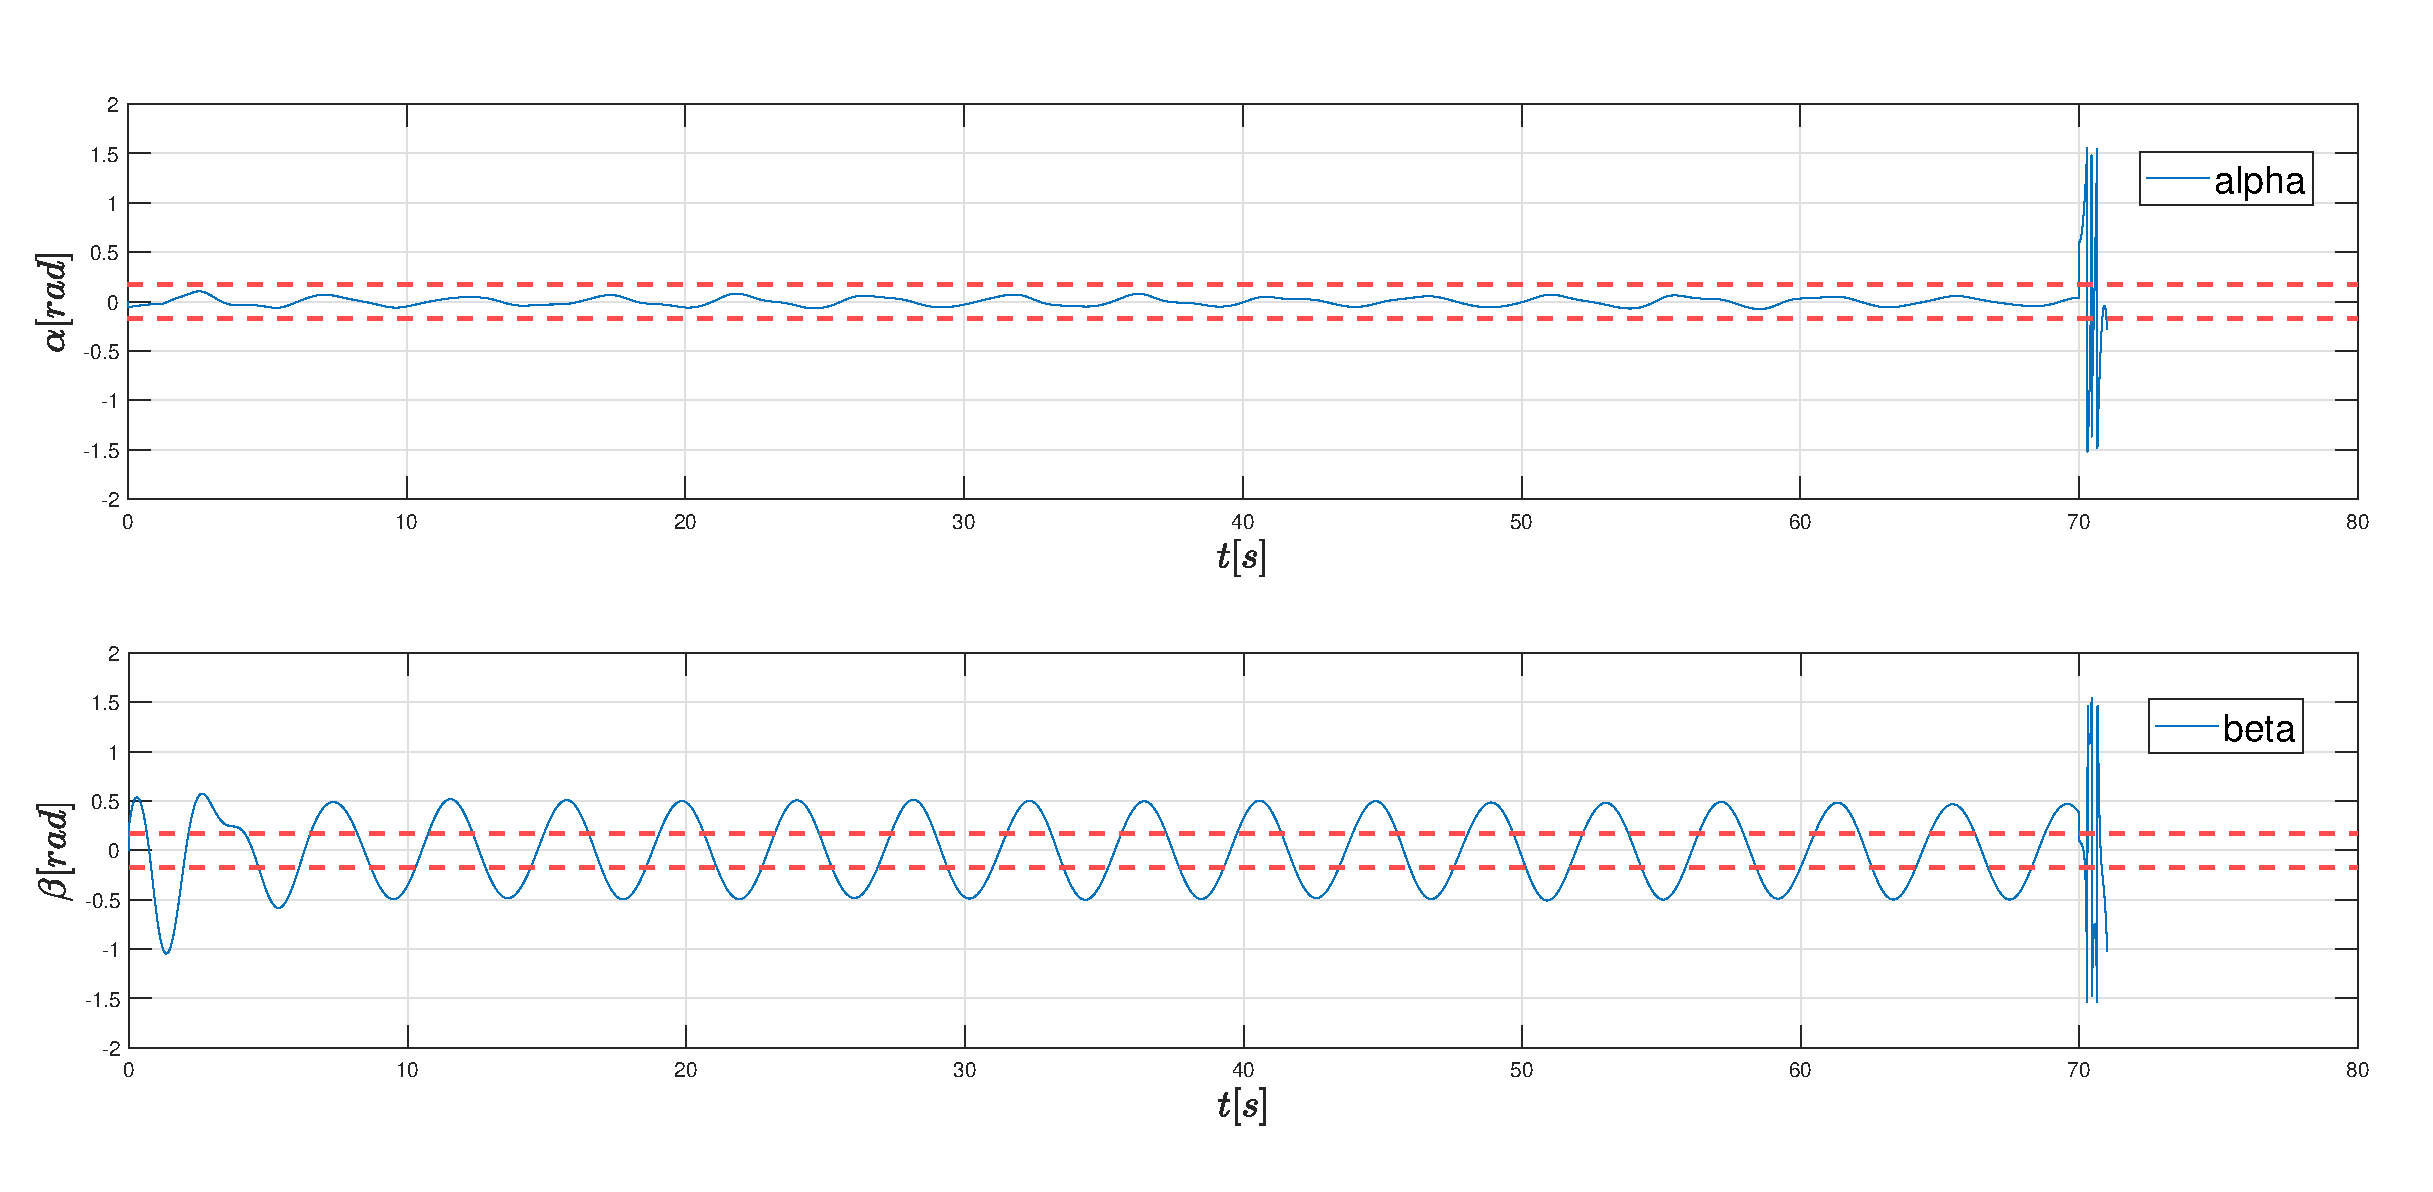
\includegraphics[scale=0.2]{figures/FL_angles}
    \caption{Angles $\alpha$ and $\beta$ of the swashplate.}
    \label{fig:FL_angles}
\end{figure}
\begin{figure}[H]
    \centering
    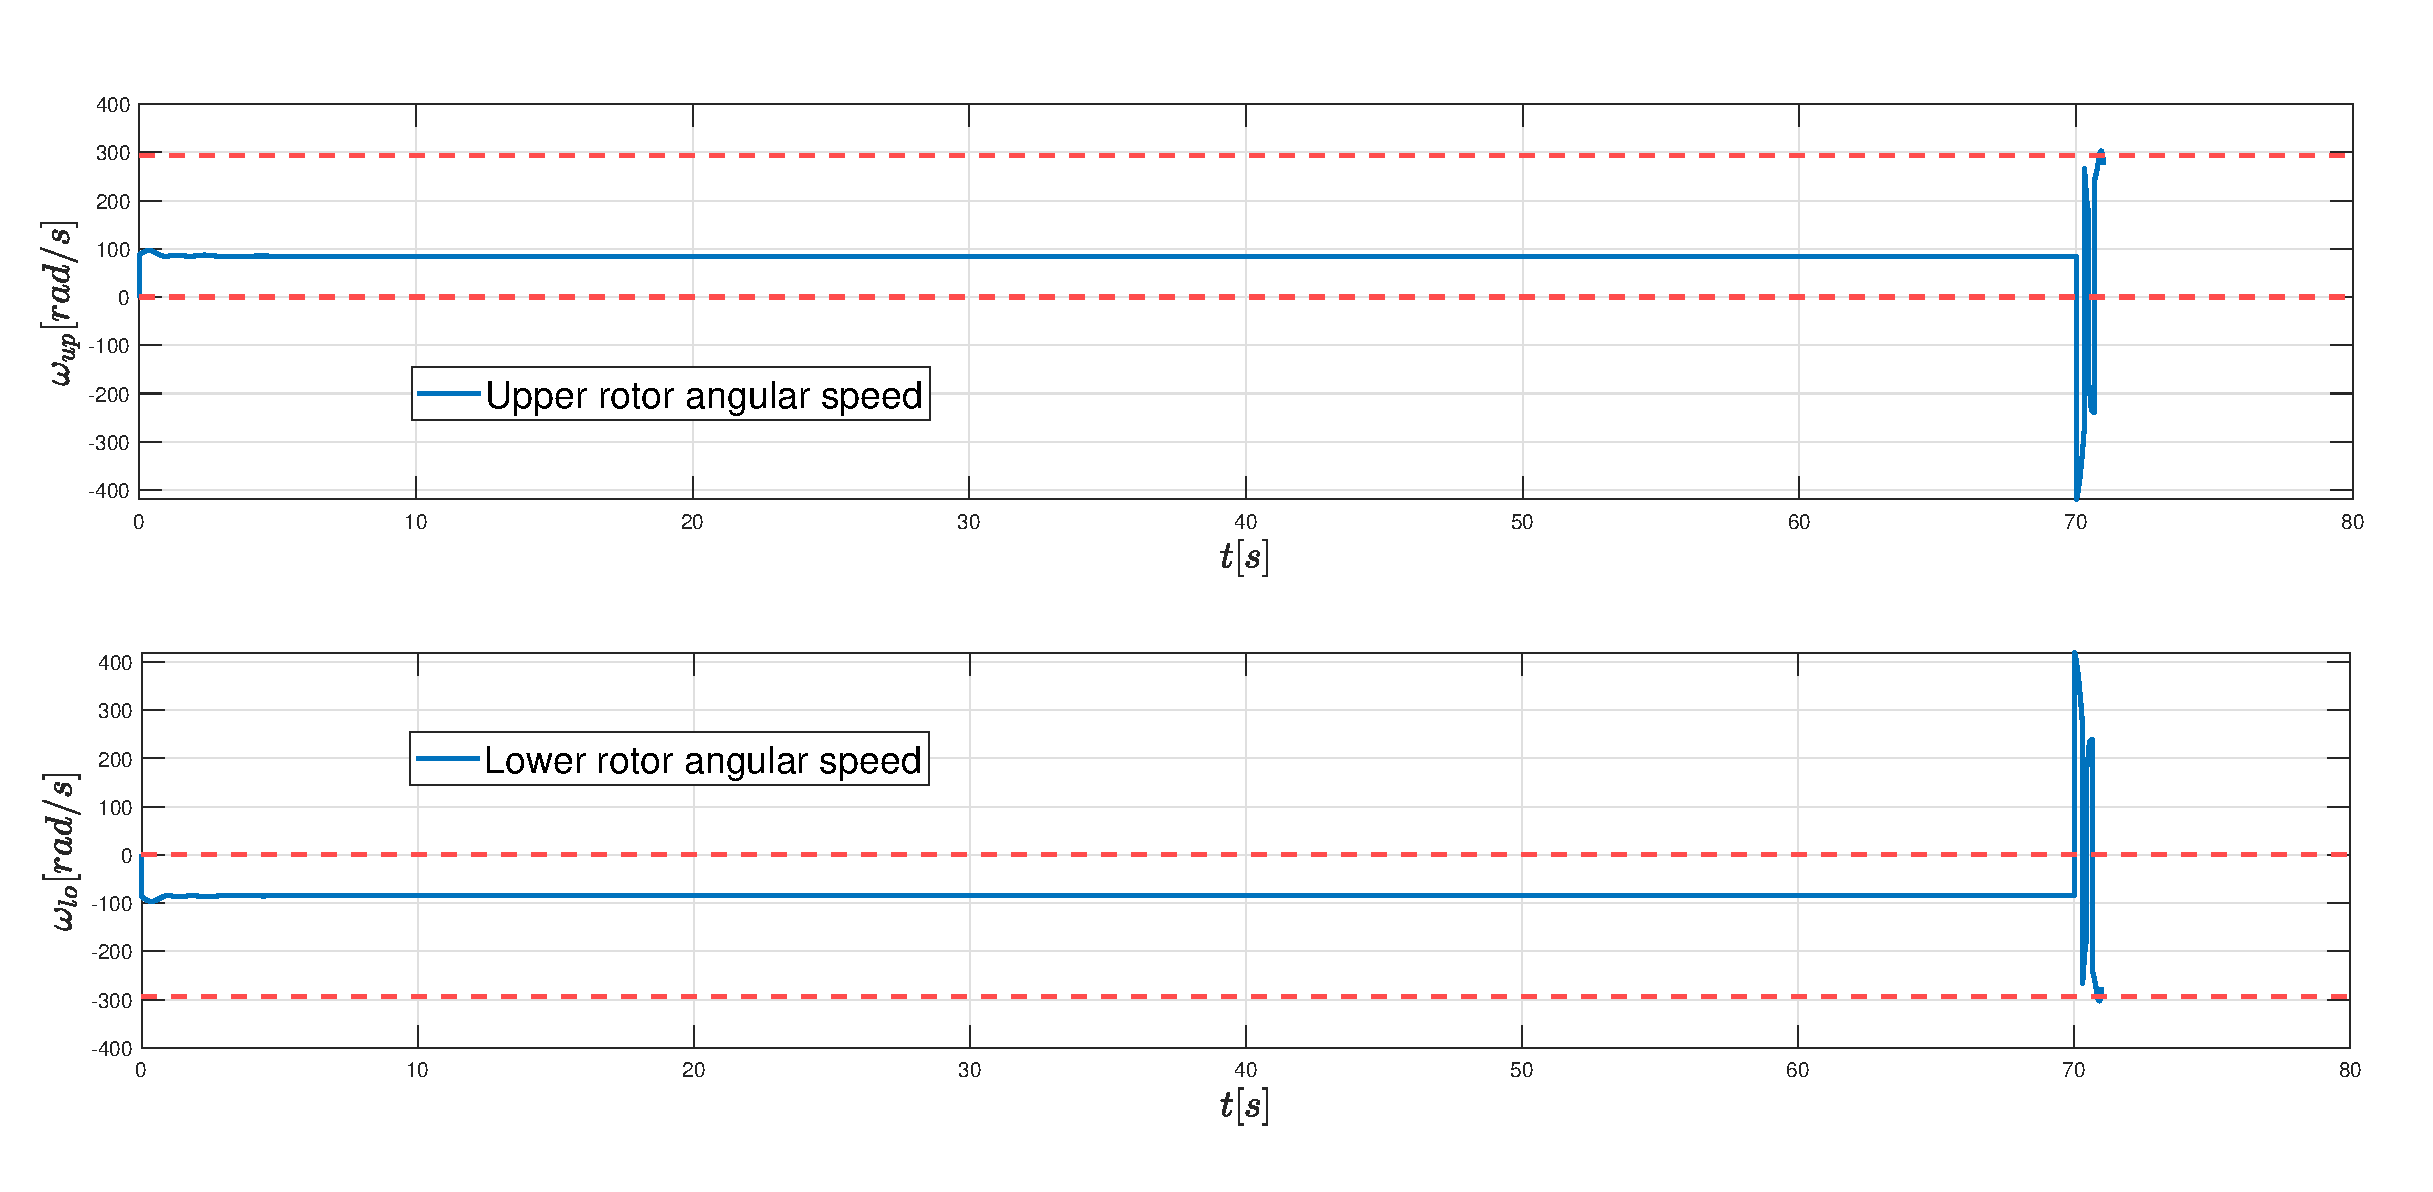
\includegraphics[scale=0.2]{figures/FL_omega}
    \caption{Angular velocities of the upper and lower rotor respectively.}
    \label{fig:FL_omega}
\end{figure}

